% Options for packages loaded elsewhere
\PassOptionsToPackage{unicode}{hyperref}
\PassOptionsToPackage{hyphens}{url}
%
\documentclass[
]{article}
\usepackage{amsmath,amssymb}
\usepackage{lmodern}
\usepackage{ifxetex,ifluatex}
\ifnum 0\ifxetex 1\fi\ifluatex 1\fi=0 % if pdftex
  \usepackage[T1]{fontenc}
  \usepackage[utf8]{inputenc}
  \usepackage{textcomp} % provide euro and other symbols
\else % if luatex or xetex
  \usepackage{unicode-math}
  \defaultfontfeatures{Scale=MatchLowercase}
  \defaultfontfeatures[\rmfamily]{Ligatures=TeX,Scale=1}
\fi
% Use upquote if available, for straight quotes in verbatim environments
\IfFileExists{upquote.sty}{\usepackage{upquote}}{}
\IfFileExists{microtype.sty}{% use microtype if available
  \usepackage[]{microtype}
  \UseMicrotypeSet[protrusion]{basicmath} % disable protrusion for tt fonts
}{}
\makeatletter
\@ifundefined{KOMAClassName}{% if non-KOMA class
  \IfFileExists{parskip.sty}{%
    \usepackage{parskip}
  }{% else
    \setlength{\parindent}{0pt}
    \setlength{\parskip}{6pt plus 2pt minus 1pt}}
}{% if KOMA class
  \KOMAoptions{parskip=half}}
\makeatother
\usepackage{xcolor}
\IfFileExists{xurl.sty}{\usepackage{xurl}}{} % add URL line breaks if available
\IfFileExists{bookmark.sty}{\usepackage{bookmark}}{\usepackage{hyperref}}
\hypersetup{
  pdftitle={La mortalité en Europe},
  pdfauthor={Pierre Décoder l'éco},
  hidelinks,
  pdfcreator={LaTeX via pandoc}}
\urlstyle{same} % disable monospaced font for URLs
\usepackage[margin=1in]{geometry}
\usepackage{graphicx}
\makeatletter
\def\maxwidth{\ifdim\Gin@nat@width>\linewidth\linewidth\else\Gin@nat@width\fi}
\def\maxheight{\ifdim\Gin@nat@height>\textheight\textheight\else\Gin@nat@height\fi}
\makeatother
% Scale images if necessary, so that they will not overflow the page
% margins by default, and it is still possible to overwrite the defaults
% using explicit options in \includegraphics[width, height, ...]{}
\setkeys{Gin}{width=\maxwidth,height=\maxheight,keepaspectratio}
% Set default figure placement to htbp
\makeatletter
\def\fps@figure{htbp}
\makeatother
\setlength{\emergencystretch}{3em} % prevent overfull lines
\providecommand{\tightlist}{%
  \setlength{\itemsep}{0pt}\setlength{\parskip}{0pt}}
\setcounter{secnumdepth}{-\maxdimen} % remove section numbering
\ifluatex
  \usepackage{selnolig}  % disable illegal ligatures
\fi

\title{La mortalité en Europe}
\author{Pierre Décoder l'éco}
\date{20/05/2021}

\begin{document}
\maketitle

{
\setcounter{tocdepth}{2}
\tableofcontents
}
\hypertarget{comprendre-les-donnuxe9es-de-mortalituxe9-europuxe9enne-pour-prendre-les-bonnes-duxe9cisions}{%
\section{Comprendre les données de mortalité européenne pour prendre les
bonnes
décisions}\label{comprendre-les-donnuxe9es-de-mortalituxe9-europuxe9enne-pour-prendre-les-bonnes-duxe9cisions}}

\hypertarget{la-nuxe9cessituxe9-de-saffranchir-des-biais-de-perception}{%
\subsection{La nécessité de s'affranchir des biais de
perception}\label{la-nuxe9cessituxe9-de-saffranchir-des-biais-de-perception}}

Cet article a pour objectif d'analyser les données de mortalité de 33
pays européens afin de comprendre les dynamiques en jeu depuis plus d'un
an.

Toutes les données utilisées proviennent de sources officielles~:

\begin{itemize}
\item
  Eurostat pour les décès et la population par âge des pays européens
\item
  Insee pour les données détaillées françaises
\item
  Ourworldindata pour les données de malades, décès et vaccination en
  lien avec la Covid 19
\item
  Médicam pour les données des médicaments délivrés les les pharmacies
  de ville
\item
  Ecdc pour les données des mesures prises par les différents pays
\end{itemize}

Toutes les données de mortalité utilisées dans cet article, sont des
données de mortalité toutes causes confondues et pas uniquement des
données de mortalité de la seule cause Covid-19. En effet pour
considérer qu'une maladie est mortelle, il faut qu'elle ait un impact
sur la mortalité générale, et pas uniquement compter les décès de
personnes qui en sont porteuses. Chacun conviendra que cela n'aurait
aucun sens statistique de compter les décès survenus après la
dégustation d'une glace à la vanille. Pourtant en le faisant nous
verrions une forte augmentation de ces décès l'été, uniquement parce
qu'en France 1500 personnes décèdent tous les jours l'été, et qu'à cette
période, elles dégustent plus souvent des glaces à la vanille. Il s'agit
de ce que l'on appelle un biais de perception.

Le fait de présenter en permanence des statistiques de mortalité de
personnes porteuses de la Covid induit un biais de perception. Il laisse
imaginer que ce virus est la seule cause de mortalité aujourd'hui sans
jamais confronter ces décès au nombre de décès habituels de chaque pays.
Dans ce contexte, il est impossible de réaliser une recherche
raisonnable des causes de décès depuis mars 2020 : c'est la Covid-19 qui
s'impose et rien d'autre n'est envisageable. C'est le contraire d'une
démarche scientifique.

Pour cette raison, cet article se base uniquement sur les décès toutes
causes et met en lien les différents évènements et choix qui ont été
pris dans les différents pays, afin de chercher des causes de décès sans
biais préalable.

Les données des décès toutes causes sont étonnamment et malheureusement
beaucoup plus difficiles à trouver. On ne peut qu'être surpris de
constater qu'elles ne bénéficient pas de la diffusion des statistiques
de la Covid et ses nombreux sites internet redoublant d'interfaces
graphiques. Elles doivent être téléchargées sur des sites spécialisés et
retravaillées pour les rendre exploitables. Elles sont pourtant les
seules permettant une analyse objective de la situation. Il
``suffirait'' pourtant à des sites tels qu'Ourworldindata de se
``brancher'' sur les sites officiels de dépôts de données statistiques
tels qu'Eurostat pour proposer des graphiques et animations éclairant le
débat sur de nombreux sujets. Eurostat propose même une interface de
programmation d'application (API) permettant à toute personne de
télécharger et d'utiliser n'importe quelle base de données.

Concernant Ourworldindata, il ne s'agit pas d'un problème de ``place''
puisque le site héberge déjà 300 thèmes et plus de 3000 visualisations
de données. Il s'agit d'un choix éditorial. Les thèmes et graphiques
proposés dans tout exercice de communication correspondent à des choix
discutés et validés. Sur Ourworldindata, les données mises en valeur
sont actuellement représentatifs des centres d'intérêts politiques et
médiatiques aujourd'hui : croissance de la population, espérance de vie,
pollution, dépenses gouvernementales, corruption et bien évidemment
Covid-19. Il s'agit bien d'un site de communication dont l'enjeu est de
convaincre (ou persuader), et non pas un site de recherche dont le but
est de questionner pour comprendre.

Cet article présente en première partie le bilan de l'année 2020 pour
montrer que dans sa globalité, cette année est loin d'être
exceptionnelle du point de vue de la mortalité. Ce résultat est confirmé
pour tous les pays d'Europe pour lesquels nous avons des données de
population et de décès.

En seconde partie, cet article présente les décès semaine après semaine
de tous les pays européens. Pour comprendre les dynamiques en jeu, 3
périodes de mortalité liées à la Covid-19 seront étudiées~:

\begin{itemize}
\item
  la période de mars-avril 2020, spécifique à un nombre restreint de
  pays européens
\item
  la période d'octobre à décembre 2020 qui présente une hausse des décès
  inhabtiuelle
\item
  la période depuis début 2021 qui présente un rebond de mortalité
  lui-aussi inhabituel
\end{itemize}

Nous verrons que dans les 3 cas, la mortalité est liée non pas à la
seule présence d'une nouvelle maladie, mais directement aux choix de
politiques sanitaires pris. Dans tous les cas, la croyance dans des
modèles de propagation épidémique a induit les pouvoirs publics en
erreur. La lutte contre la propagation au détriment de la qualité des
soins s'est finalement révélée catastrophique. Cette expérience prouve
que les modèles épidémiques utilisés sont déconnectés de la réalité et
que seule la qualité du soin prévaut. Au regard des données collectées
de mortalité, nous questionnons la stratégie de santé mise en place
depuis plus d'un an, du port du masque au confinement total et jusqu'au
pari vaccinal au détriment du soin classique.

\hypertarget{du-point-de-vue-de-la-mortalituxe9-lannuxe9e-2020-est-comparable-au-reste-de-la-duxe9cennie-pour-une-majorituxe9-de-pays-deurope}{%
\subsection{1. Du point de vue de la mortalité, l'année 2020 est
comparable au reste de la décennie pour une majorité de pays
d'Europe}\label{du-point-de-vue-de-la-mortalituxe9-lannuxe9e-2020-est-comparable-au-reste-de-la-duxe9cennie-pour-une-majorituxe9-de-pays-deurope}}

\hypertarget{quelques-rappels-pour-la-france-limportance-du-vieillissement-de-la-population}{%
\subsubsection{1.1 Quelques rappels pour la France~: l'importance du
vieillissement de la
population}\label{quelques-rappels-pour-la-france-limportance-du-vieillissement-de-la-population}}

Dans plusieurs vidéos de la chaîne Décoder l'éco, par exemple celle qui
compare les décès de toutes les années entre 1962 et 2020 \footnote{\url{https://youtu.be/IPu4QvUHaQE}}
nous avons vu que la mortalité en France depuis 2020 n'est pas unique et
est au niveau de l'année 2015.

En effet, la France vieillit. Ainsi le nombre de morts chaque année
augmente naturellement depuis 2010.

\includegraphics{110_la_mortalite_en_europe_files/figure-latex/unnamed-chunk-1-1.pdf}

Cette hausse du nombre de décès n'est pas le signe que la santé des
français se dégrade, mais uniquement le résultat de l'augmentation du
nombre de personnes âgées. En effet, à force de vieillir, tous les
humains finissent par mourir. Pour l'illustrer, voici la pyramide des
âges de la France en 2000 et en 2020, réalisée avec les données
disponibles sur Eurostat.

\includegraphics[width=4.6875in,height=\textheight]{gen/images/pyramid_france_2000.png}
\includegraphics[width=4.6875in,height=\textheight]{gen/images/pyramid_france_2020.png}
En 20~ans, la génération des baby-boomers est, logiquement, passée de la
tranche des moins de 55~ans à celle des plus de 65~ans. Dès lors, il est
tout à fait normal que le nombre de décès en France augmente chaque
année, et cela va continuer à augmenter pendant encore au moins 20~ans.

Ainsi, il ne faut jamais commenter des nombres de décès bruts qui
augmentent ou baissent non pas selon l'arrivée des maladies, mais
toujours selon la taille de la population et selon l'âge des personnes.
En effet, s'il y a plus de décès en France qu'au Luxembourg, c'est parce
que les français sont 100 fois plus nombreux que les Luxembourgeois.
S'il y a plus de décès dans un EHPAD de 200~personnes que dans une école
maternelle de 200~enfants, ce n'est pas parce que l'EHPAD est plus
dangereux que l'école maternelle, mais uniquement parce que les
résidents d'un EHPAD sont beaucoup plus vieux que les élèves d'une école
maternelle. Ainsi, comparer des nombres de décès entre 2 populations ne
peut pas se faire avec les seuls chiffres bruts, mais toujours en
corrigeant de la taille de la population, et aussi en corrigeant de
l'âge des gens. Il s'agit de standardiser les décès pour mettre la même
population partout.

Pour comparer le nombre de décès en France de ces dernières années avec
l'année 2020, nous avons standardisé les décès, en appliquant la
population par âge de 2020 à toutes les années du passés. Il en est
ressorti que l'année 2020 n'est pas du tout une année de record de
mortalité.

\includegraphics{110_la_mortalite_en_europe_files/figure-latex/unnamed-chunk-2-1.pdf}

L'année 2020 est au niveau de l'année 2015. Il s'agit de la 6e année la
moins mortelle de toute l'histoire de la France. Dès lors, on ne peut
justifier une panique sanitaire et des mesures exceptionnelles sur la
base des décès de l'année 2020 en France.

Cette situation est la même quel que soit le pays en Européen considéré.

\hypertarget{lannuxe9e-2020-en-europe-une-annuxe9e-dans-la-norme-pour-tous-les-pays}{%
\subsubsection{1.2 L'année 2020 en Europe~: Une année dans la norme pour
tous les
pays}\label{lannuxe9e-2020-en-europe-une-annuxe9e-dans-la-norme-pour-tous-les-pays}}

Tous les pays européens vivent au rythme des nouvelles annonces et
mesures concernant la Covid-19 depuis plus d'un an. Mais qu'en est-il
réellement du point de vue de la mortalité~? L'année 2020 est-elle
vraiment une année d'hécatombe quelque part~? Cette carte d'Europe
représente l'année pour laquelle chaque pays européen, dont nous
disposons des données, a connu le plus de décès.

En marron, nous retrouvons tous les pays pour lesquels l'année 2020 est
l'année pour laquelle il y a eu le plus de décès. C'est bien le cas de
la majorité des pays d'Europe. On note toutefois quelques exceptions, en
particulier les pays nordiques. Cette carte est réalisée avec des
données brutes. Comme nous l'avons vu pour la France, les données brutes
reflètent avant tout l'augmentation et le vieillissement de la
population.

La pyramide des âges des pays Européens révèle une situation européenne
semblable à celle de la France : la population vieillit. Il est tout à
fait normal que le nombre de décès augmente chaque année du fait de ce
simple constat.

\includegraphics[width=4.6875in,height=\textheight]{gen/images/pyramide_europe_2000.png}
\includegraphics[width=4.6875in,height=\textheight]{gen/images/pyramide_europe_2020.png}

Ainsi, plutôt que de regarder les décès bruts, il est nécessaire de les
corriger par la pyramide des âges, de façon à prendre en compte
l'augmentation et le vieillissement de la population dans les calculs.
Cela permet de ne pas dire que la mortalité augmente, si cela vient
juste du fait qu'il y a plus de personnes âgées.

En calculant pour chaque pays, les décès standardisés par âge, pour
toutes les années, il est désormais possible de les comparer aux décès
2020. Cela permet de savoir si à population égale, l'année 2020 a été
réellement plus mortelle que les autres. Ce calcul, permet de déger 5
profils type de pays représentés sur cette carte.

Pour l'Islande, la Norvège et le Danemark , l'année 2020 est en fait
l'année la moins mortelle de toute leur histoire. Dans ces pays, les
habitants ne sont jamais moins morts qu'en 2020. Ce n'est pas pour
autant qu'ils n'ont pas de morts attribués à la Covid-19,~mais dans ces
pays, malgré la pandémie annoncée, l'année 2020 est le record absolu de
plus faible mortalité.

L'Allemagne, la Suède, la Finlande, l'Estonie et la Lituanie ont vécu la
2e année la moins mortelle de toute leur histoire. Seule l'année 2019 a
enregistré moins de décès. En effet, pour l'écrasante majorité des pays
d'Europe, l'année 2019 a été un record de sous-mortalité qui sera très
difficile à battre, même en enfermant toute la population.

Une majorité des pays d'Europe, dont la France, a vécu une année 2020
dans la norme de la décennie. Les pays en orange clair sont plutôt dans
la 2e moitié de la décennie, autour des années 2015-2016. Les pays en
orange foncé sont plus souvent autour de l'année 2012.

Seuls l'Espagne, l'Italie, la Belgique, la Roumanie, la Bulgarie la
Pologne et le Monténégro ont connu une mortalité forte pour la décennie.
Ainsi, les pays d'Europe ayant connu les plus fortes mortalités
relativement à ce qu'ils enregistrent habituellement, ont connu une
mortalité de l'ordre de la 10e plus faible de toute leur histoire.

L'année 2020 présentée comme une hécatombe mondiale, n'est en fait
qu'une année pendant laquelle, au pire, les humains sont morts dans les
mêmes proportions que l'année 2010. Ce qui est montré depuis 6 mois pour
la France sur la chaîne Décoder l'éco, est donc réplicable pour tous les
pays pour lesquels des données sont disponibles.

Au bilan, pas un seul pays d'Europe n'a vécu une ``hécatombe'' en 2020.
Pour les pire cas, 2020 est juste aussi mortelle que 2010.

\hypertarget{la-mortalituxe9-en-europe-le-pays-de-ruxe9sidence-bien-plus-duxe9terminant-que-lannuxe9e}{%
\subsubsection{1.3 La mortalité en Europe : le pays de résidence bien
plus déterminant que
l'année}\label{la-mortalituxe9-en-europe-le-pays-de-ruxe9sidence-bien-plus-duxe9terminant-que-lannuxe9e}}

Nous venons de voir qu'en corrigeant les décès de la pyramide des âges
de chaque pays, on montre que 2020 est finalement une année mortalité
dans la norme de la décennie. Afin de compléter notre vision, il est
important de comparer les pays entre eux. Seulement les populations des
pays européens sont trop différentes pour être comparables. Entre
l'Allemagne et ses 83 millions d'habitants et le Liechtenstein et ses 38
000 habitants, il est impossible de faire un graphique à la même
échelle. Il est donc nécessaire de les comparer sur une même base. Pour
ce faire, nous allons appliquer la même pyramide des âges à tous les
pays Européens. Ainsi nous pourrons savoir, dans quel pays et pendant
quelle année, les européens sont le plus décédés.

Ces graphiques représentent les décès théorique pour chaque pays et
chaque année, s'ils avaient eu la population et la pyramide des âges de
la France en 2020. Il sont séparés entre les pays de l'Est et les pays
de l'Ouest de l'Europe pour une question de visibilité, mais également
parce que ces 2 zones de l'Europe sont assez différentes du point de vue
de la mortalité.

Les décès théoriques de 2020 pour chaque pays sont signalés en rouge et
les autres points en dégradé de bleu représentent les décès théoriques
des autres années.

Par exemple, si la population de la France de 2020 étaient décédée de la
même manière que la Bulgarie en 2020, il y aurait eu 1 300 000 morts au
lieu des 660 000 qu'elle a vécu.

\includegraphics[width=10.41667in,height=\textheight]{gen/images/deces2000est.png}
\includegraphics[width=10.41667in,height=\textheight]{gen/images/deces2000ouest.png}

Cela montre qu'à population et pyramide des âges égales, les bulgares
meurent deux fois plus que les français.

Ainsi, si la Bulgarie n'a pas 2 fois plus de morts que la France chaque
année, c'est d'abord parce que les Bulgares sont 7 millions et les
français 67 millions, mais aussi parce que les Bulgares sont plus jeunes
que les français.

Les Bulgares sont plus jeunes que les français notamment parce qu'ils
meurent plus jeunes. Il y a donc moins de personnes dans leur population
qui peuvent arriver à des âges avancés. Ils décèdent petit à petit plus
fortement que les français.

Les différences de mortalité d'une année à l'autre sont parfaitement
négligeables devant les différences d'un pays à l'autre. La probabilité
de décéder à chaque âge dépend avant tout de l'endroit où l'on vit et
moins des années.

Si on se met à la place d'un Bulgare. Grace à se graphique, nous
apprenons que la mortalité en Bulgarie est 2 fois plus élevée que celle
de la France à population égale. Ne faudrait-il pas se dire qu'il y a
certainement des choses à faire sur la pauvreté et la santé en Bulgarie
pour se rapprocher de la situation de la France. Nous constatons que la
Bulgarie constate juste une augmentation de 10\% de mortalité en 2020
par rapport à 2019, pour se retrouver au niveau de la mortalité de
l'année 2015, et que cela est sensé déclencher une énorme panique. En
nombre de décès standardisé, c'est comme si chaque année, la Bulgarie
avait 500 000 morts de plus que la France, et qu'elle trouvait ça tout à
fait normal, mais qu'elle paniquait en 2020 pour 100 000 morts de plus
que 2019.

C'est comme si un éléphant et une colonie de fourmis montaient sur un
bateau, que le bateau se mettait à couler et que l'éléphant réussissait
à convaincre les fourmis de sauter une à une du bateau jusqu'à ce qu'il
flotte de nouveau.

Ce graphique montre que les évènements particuliers ont peu d'impact sur
la mortalité et que ce sont les effets structurels, de la santé des
habitants et de la qualité du système de santé qui prévalent.

Ce graphique montre également que les français vivent dans l'un des pays
d'Europe, et donc du monde, au sein duquel on meurt le moins.

Nous avons montré plus haut que l'année 2020 est la 6e année pour
laquelle les français sont le moins mort. Ce graphique nous montre que
la mortalité de la France en 2020 a été une des plus faibles jamais
enregistrée dans tous les pays du monde. Pour la quasi totalité des
humains ayant jamais vécu sur cette planète, l'année 2020 en France est
l'un des endroits et moment où on a connu le moins de morts.

Il n'est donc à aucun moment justifiable de générer une panique et des
mesures d'une ampleur colossale pour des décès qui ne sont nulle part
exceptionnels, et surtout pas en France.

\hypertarget{une-baisse-de-mortalituxe9-aujourdhui-nentrauxeene-pas-une-baisse-de-la-mortalituxe9-demain}{%
\subsubsection{1.4 Une baisse de mortalité aujourd'hui n'entraîne pas
une baisse de la mortalité
demain}\label{une-baisse-de-mortalituxe9-aujourdhui-nentrauxeene-pas-une-baisse-de-la-mortalituxe9-demain}}

De nombreuses études commentent l'année 2020 au regard de son
augmentation par rapport à 2019. Ces études considèrent que la baisse de
mortalité observée ces dernières années et tout particulièrement en 2019
doit se poursuivre. Ainsi, les morts en plus de l'année 2020 sont
considérées comme une catastrophe évitable attribuée à un virus.

Seulement, imaginer que la baisse de mortalité peut se poursuivre
indéfiniment revient tout bonnement à nier que les humains finissent par
mourir.

L'année 2019 a connu une mortalité extrêmement faible partout en Europe.
Il semble banal de penser que si des morts sont évités une année, elles
finiront par se répercuter sur les années suivantes et non pas ne plus
jamais survenir. Encore en 2020, on ne peut pas éviter la mort, au mieux
on la repousse.

Si on imagine un cas théorique où on trouverait un territoire sur lequel
personne n'est mort pendant une année. Il ne viendrait à l'idée de
personne que les habitants de ce territoire vivraient éternellement.
Pourtant, la projection de la mortalité de ce territoire supposerait
qu'il n'y ait pas de morts non plus l'année suivante. Avec cette
méthode, tout mort serait alors suspect et compté comme de la
surmortalité.

Ce cas trivial est pourtant ce qui est fait lorsque l'on compare l'année
2020 à la seule année 2019, ou que l'on essaye de continuer de faire
baisser indéfiniment des taux de mortalité.

Sur le graphique du nombre de décès français, on observe certaines
années plus ou moins élevées par rapport à la tendance générale. Dans la
littérature, les années de fortes mortalité sont appelées années
moissons.

\includegraphics{110_la_mortalite_en_europe_files/figure-latex/unnamed-chunk-3-1.pdf}

Ces années apparaissent tous les 2 à 3 ans. Ainsi, pour comprendre si
les décès d'une année ont un impact visible sur une période, une méthode
peut consister à regarder les décès sur 3 années consécutives. Le
dernier trio d'années, 2018-2019-2020 est en rouge pour plus de
visibilité.

\includegraphics[width=10.41667in,height=\textheight]{gen/images/deces3annees.png}

Sans surprise, pour la quasi-totalité des pays européens, il n'est
jamais décédé aussi peu de personnes relativement à leur âge que ces
3~dernières années. L'année 2020 n'a pas entièrement contrebalancé les
faibles mortalités des années 2018 et 2019.

\hypertarget{la-chute-de-lespuxe9rance-de-vie-nest-quune-autre-maniuxe8re-de-pruxe9senter-le-muxeame-ruxe9sultat}{%
\subsubsection{1.5 La chute de l'espérance de vie n'est qu'une autre
manière de présenter le même
résultat}\label{la-chute-de-lespuxe9rance-de-vie-nest-quune-autre-maniuxe8re-de-pruxe9senter-le-muxeame-ruxe9sultat}}

Le 19 janvier 2021, l'Insee a sorti son bilan démographique de l'année
2020 \footnote{\url{https://www.insee.fr/fr/statistiques/5012724}} en
décidant de mettre comme titre « Avec la pandémie de Covid-19, nette
baisse de l'espérance de vie et chute du nombre de mariages ». Bien
évidemment, la presse s'est emparée de ce titre pour expliquer à quel
point la situation était grave. Les journalistes ont bien évidemment
déduit du titre de l'Insee, que les français ont vécu moins longtemps
que d'habitude, et qu'en plus cette diminution était causée par la
Covid-19.

D'ailleurs, un des sous-titres de l'article de l'Insee est directement
``En 2020, la pandémie a fait perdre 0,4 an d'espérance de vie aux
femmes et 0,5 an aux hommes''. Ainsi le lien est direct : c'est la
pandémie qui tue.

La vidéo dédiée sur la chaîne Décoder l'éco \footnote{\url{https://youtu.be/UKpOOtnCnCQ}}
détaille le calcul de l'espérance de vie. Cet indicateur fait partie de
la famille des agrégats. C'est-à-dire qu'il est construit en
additionnant des choses qui vont dans tous les sens et finalement ne
renseigne pas du tout sur ce qu'il se passe vraiment. Il a juste un joli
nom induisant les gens en erreur, pensant avoir compris ce qu'il
signifie.

Le mot « espérance » est un terme utilisé en mathématiques qui signifie
« moyenne sur un grand nombre de fois », en tenant compte de la
pondération comme toute moyenne. Par exemple lorsque vous lancez 2 dés à
6 faces, et que vous additionnez le nombre de points sur vos 2 dés, en
moyenne, vous faites 7, votre espérance mathématique est 7. On ne
connaît pas le résultat de votre prochain lancé. L'indicateur «
espérance de vie » n'est donc pas du tout à entendre au sens de « espoir
» et encore moins « nombre d'années que vous pouvez espérer vivre ».
L'espérance de vie ne vous renseigne pas du tout sur votre avenir, mais
est juste une image du présent. L'espérance de vie 2020, est une moyenne
standardisée de l'âge des gens morts en 2020. Elle nous donne une idée
de l'âge des morts en 2020, en tenant compte de la structure par âge.
L'espérance de vie 2020 ne correspond absolument pas à l'âge que vous
pourrez espérer vivre. Si vous lisez cet article, vous n'êtes pas morts
en 2020. Vous ne jouez pas avec les mêmes dés que ceux qui sont morts en
2020 ou avant.

Dans le présent article nous utilisons une autre forme de
standardisation que l'espérance de vie. Elle donne exactement la même
conclusion que celle de l'article de l'INSEE. Sur l'article de l'INSEE
nous pouvons lire que l'espérance de vie 2020 est la même que
l'espérance de vie 2015, sur notre article nous concluons que les décès
standardisés de 2020 sont aussi nombreux qu'en 2015. Se focaliser sur la
chute plutôt que sur le niveau, et sur le terme ``espérance de vie''
sans l'expliquer n'est qu'un choix éditorial et pas une analyse
approfondie.

\hypertarget{des-pics-de-mortalituxe9s-uxe0-relier-aux-duxe9cisions-prises-depuis-2020}{%
\subsection{2 Des pics de mortalités à relier aux décisions prises
depuis
2020}\label{des-pics-de-mortalituxe9s-uxe0-relier-aux-duxe9cisions-prises-depuis-2020}}

Depuis le début de l'année 2020, des décisions inédites ont été prises
en France et dans beaucoup de pays du monde. Ces décisions avaient pour
objectif de diminuer le nombre de décès. Nous avons vu dans la première
partie de cet article que finalement, la mortalité de 2020 ne présente
pas d'anomalie alarmante lorsqu'elle est prise dans son ensemble et
comparée aux années de la dernière décennie. Il convient cependant pour
mieux comprendre les mécanismes en jeu depuis plus d'un an, et étudier
finement les décès hebdomadaires des pays européens et de les confronter
aux mesures prises.

\hypertarget{la-mortalituxe9-hivernale-nest-pas-un-phuxe9nomuxe8ne-de-propagation}{%
\subsubsection{2.1 La mortalité hivernale n'est pas un phénomène de
propagation}\label{la-mortalituxe9-hivernale-nest-pas-un-phuxe9nomuxe8ne-de-propagation}}

L'étude de la carte des décès hebdomadaires standardisés en France
depuis 2013 nous permet de visuliser les cycles de mortalité.
\includegraphics[width=10.41667in,height=\textheight]{gen/images/deceshebdofrance.png}

Chaque année, le nombre de décès augmente en hiver et diminue en été.
Cette augmentation de décès l'hiver est concomitante des maladies
hivernales, dont les infections respiratoires aiguës comme les grippes
ou les coronavirus.

Certains hivers présentent des pics de mortalité nettement supérieurs à
d'autres. L'hiver 2013-2014 a connu des pics de mortalité bien moins
élevés que l'hiver 2014-2015. Cette différence fait partie des éléments
expliquant les différences de décès d'une année sur l'autre. De plus,
certaines années les pics de décès peuvent être plus ou moins précoces
ou tardifs. L'année 2017 supporte ainsi la majorité de la mortalité de
l'hiver 2016-2017, mais également une importante partie de celle de
l'hiver 2017-2018. Ainsi, le décalage des mortalités hivernales
entraînent des différences de nombres de décès sur l'année.

Le découpage annuel n'est donc pas le plus adapté pour étudier la
mortalité, car il découpe la mortalité hivernale de manière inégale
selon les années. Il est cependant le plus facile à représenter, car
correspond aux données administratives et statistiques.

Ce phénomène de mortalité hivernale est complètement simultané sur toute
l'Europe. La standardisation des décès nous permet de représenter les
différents pays et années sur un même graphique.

\includegraphics[width=10.41667in,height=\textheight]{gen/images/deceshebdofrancesuedeportugal.png}
De la Suède jusqu'au Portugal, les hausses de mortalité sont
naturellement simultanées tous les hivers, et même les étés lors des
épisodes caniculaires. La mortalité hivernale des pays européens n'est
donc pas en lien avec un phénomène de diffusion de maladies l'hiver en
Europe. Le Portugal et la Suède sont séparés par 3000 km. Si la
diffusion entre individus de maladies l'hiver était responsable de
l'augmentation de la mortalité, de décalages temporels devraient être
visibles, ce qui n'est pas le cas. L'augmentation des décès ne
représente pas le déplacement des maladies, mais leur apparition partout
à la fois. Il s'agit d'une manifestation de la dégradation cyclique de
l'état de santé. Cette dégradation simultanée partout en Europe se
traduit par l'apparition de symptômes attribués à des maladies
hivernales et par l'augmentation des décès. Le phénomène de courbe en
cloche concernant la mortalité n'est pas le résultat d'un phénomène de
propagation, mais d'une phénomène d'apparition. Il est évident que les
portugais ne contaminent pas les suédois, ni inversement.

Le même résulat se constate à des niveaux plus fins que les pays. En
France, pour lequel nous avons des résultats départementaux, les pics de
mortalité sont synchronisés. Ils sont plus ou moins visibles selon l'âge
et la taille de la population.

\hypertarget{le-pic-de-mortalituxe9-de-mars-avril-2020-ne-concerne-que-peu-de-territoires}{%
\subsubsection{2.2 le pic de mortalité de mars-avril 2020 ne concerne
que peu de
territoires}\label{le-pic-de-mortalituxe9-de-mars-avril-2020-ne-concerne-que-peu-de-territoires}}

Contrairement à une idée largement répandue, le phénomène de pic de
mortalité aux mois de mars-avril 2020 n'est absolument pas un phénomène
mondial. Sur les 33 pays étudiés dans cet article, seuls 9 présentent
une mortalité supérieure à la mortalité habituelle sur cette période :
la Belgique, la Suisse, Chypre, l'Espagne, la France, l'Italie, le
Luxembourg, les Pays-bas et la Suède (cf.~annexes)

Ce phénomène très limité doit alors s'analyser au regard de la situation
particulière de chaque pays et surtout des mesures spécifiques prises
sur la période. Cet article présente les liens trouvés entre la hausse
de la mortalité française et les mesures exceptionnelles prises.

Au niveau des départements français, le pic de mortalité de mars-avril
2020 n'a touché ni tous les territoires, ni avec la même intensité pour
tous les territoires touchés. En revanche, tous les territoires touchés
par cepix de mortalité l'ont été de manière synchronisé. Nous avons donc
un pic de mortalité qui ne touche pas tous les pays d'Europe, et au sein
de chaque pays, pas tous les territoires, mais dont tous les territoires
touchés le sont en même temps.

En Île-de-France par exemple, tous les départements connaissent une
hausse de mortalité synchronisée débutant arpès le début du confinement
identifié ici en bleu.

\includegraphics[width=10.41667in,height=\textheight]{gen/images/ÎledeFrance.png}
A l'inverse, en Nouvelle-Aquitaine, auncune hausse de mortalité n'est
visible sur la période.

\includegraphics[width=10.41667in,height=\textheight]{gen/images/NouvelleAquitaine.png}
Nous constatons également que les territoires touchés par cette hausse
de mortalité sont majoritairement des départements avec des villes de
tailles importantes (cf.~annexes) et donc des quartiers avec de très
forts taux de pauvreté. L'Insee révèle logiquement \footnote{\url{https://www.insee.fr/fr/statistiques/4627049}}
que la mortalité de cette période touche beaucoup plus fortement les
communes denses et les personnes nées à l'étranger. Il est étonnant de
la part de l'Insee qui produit les statistiques annuelles de pauvreté,
de ne pas faire le lien entre les conditions de vie et de salubrité
difficiles des quartiers pauvres, et la hausse de la mortalité. Une fois
de plus, il ne s'agit pas d'un problème de propagation, mais de santé
publique sur des territoires particuliers.

\hypertarget{le-lien-entre-les-mesures-franuxe7aises-et-les-variations-de-mortalituxe9}{%
\subsubsection{2.3 Le lien entre les mesures françaises et les
variations de
mortalité}\label{le-lien-entre-les-mesures-franuxe7aises-et-les-variations-de-mortalituxe9}}

En France, l'année 2020 comporte plus de décès que l'année 2019
notamment par la mortalité tardive visible aux mois de mars-avril, mais
également à la mortalité précoce arrivant en octobre. Un lissage des
décès sur 52 semaines, nous permet de connaître l'impact de ces
augmentations sur la mortalité habituelle.

La moyenne et les deux bornes des intervalles de confiance à 95 \%,
permettent de visualiser les périodes de mortalité anormale.

\includegraphics[width=10.41667in,height=\textheight]{gen/images/deceshebdofrancelissage.png}

Ainsi, arrivé au mois de mars 2020, la France était sur une moyenne très
basse de décès relativement aux années précédentes. Le pic de mars-avril
en France a entraîné un rapprochement vers la moyenne de décès
habituels, sans la franchir. Il s'agit donc d'un phénomène brutal avec
un impact limité. La mortalité lissée sur 52 semaines ne dépasse la
moyenne des 5 dernières années que depuis la hausse de mortalité en
octobre 2020.

Il s'agit ici de recenser les éléments qui peuvent expliquer une montée
de la mortalité en France en mars-avril 2020, de façon à évaluer ce qui
pourrait être imputable au seul virus et ce qui est imputable au reste.

En France, deux mesures structurantes concernant la politique de santé
publique ont été prises :

\begin{itemize}
\item
  Le confinement, c'est-à-dire une limitation extrême des mouvements et
  l'ordre à tous les français de rester chez eux.
\item
  L'interdiction aux médecins de ville d'appliquer leur art,
  autrement-dit de proposer des traitements pour limiter le risque de
  complication. Le débat s'est focalisé sur l'hydroxychloroquine, mais
  l'interdiction ne se limite pas à cette molécule, mais à toute
  substance en dehors du doliprane.
\end{itemize}

Ces 2 mesures ont des impacts sur l'évolution des infections
respiratoires chez les patients, mais également sur toutes les
pathologies habituelles.

\hypertarget{la-mortalituxe9-des-causes-autres-que-les-infections-respiratoires-aiguuxebs-telles-que-la-covid-19}{%
\paragraph{2.3.1 La mortalité des causes autres que les infections
respiratoires aiguës telles que la
Covid-19}\label{la-mortalituxe9-des-causes-autres-que-les-infections-respiratoires-aiguuxebs-telles-que-la-covid-19}}

Parmis les 9 pays ayant connu une surmortalité au mois de mars-avril, 7
ont mis en place un confinement à cette période. Dans tous ces pays, le
seuil de surmortalité a été franchis après le début du confinement. En
tenant compte du délai d'arrivée des données, on conclue que la décision
du confinement n'a jamais pu être déclenchée par réaction à une
surmortalité. Aucun décideur ou spécialiste ne pouvait savoir si la
période connaîtrait plus de décès qu'habituellement. La décision a été
prise notamment suite à la pression médiatique suivant des remontées de
cas Covid. Il s'agit donc d'une mesure forte qui a des impacts très
lourds sur l'organisation de la santé qui est prise avant de connaître
le niveau de danger encouru.

Il est notable qu'absolument tous les cas de figure existent en Europe,
entre confinement ou non et surmortalité ou non. Les deux effets ne sont
pas entièrement liés. Pour conclure de l'effet positif ou négatif d'une
telle mesure, il est possible de quantifier quelques effets.

Beaucoup de journaliste écrivent que le confinement strict a permis de
sauver de nombreuses vies par l'absence des accidents de voiture. Il est
aisé de quantifier le nombre de vies sauvées au maximum par une telle
mesure. Il y a environ 3 600 décès sur la route par an en France, soit
300 par mois, cela fait environ 600 décès sur la période de confinement.
Les ¾ de ces décès concernent des moins de 65 ans \footnote{\url{http://www.fiches-auto.fr/articles-auto/chiffres-infractions-securite-routiere/s-2319-nombre-d-accidents-mortels-selon-l-age-des-conducteurs.php}}.

En effet, en écrasante majorité, les personnes qui prennent leur voiture
tous les jours pour aller au travail ont moins de 65 ans. La Covid au
contraire touche les plus de 65 ans. L'impact du confinement sur la
sécurité routière aura pu sauver une partir des 600~décès possibles,
mais en écrasante majorité des jeunes, alors qu'ils ne risquent rien
avec la Covid.

Parallèlement, le 7 mai 2020, dans son bulletin épidémiologique
\footnote{\url{https://www.santepubliquefrance.fr/content/download/250807/2596023}},
Santé publique France tire la sonnette d'alarme sur le renoncement au
soin. En France, environ 120 000 infarctus sont dénombrés chaque année
\footnote{\url{https://www.frm.org/recherches-maladies-cardiovasculaires/infarctus-du-myocarde/l-infarctus-du-myocarde-en-chiffres\#:~:text=Environ\%20120\%20000\%20infarctus\%20du,d\%C3\%A9c\%C3\%A8s\%20survient\%20dans\%20l'ann\%C3\%A9e}},
soit 20 000 attendus pendant la période de confinement. De même,
150~000~AVC sont comptabilisés chaque année \footnote{\url{https://www.iledefrance.ars.sante.fr/accidents-vasculaires-cerebraux-avc\#:~:text=Chaque\%20ann\%C3\%A9e\%2C\%20plus\%20de\%2018,qui\%20gardent\%20des\%20s\%C3\%A9quelles\%20lourdes}},
soit 25 000 en 2 mois. Contrairement aux accidents de la route, les AVC
et les infarctus touchent majoritairement le même public que les
victimes de la Covid. Santé publique France nous révèle que pendant la
dernière semaine de confinement, les hôpitaux ont relevé 300 personnes
de moins aux urgences AVC et 300 personnes de moins aux urgences
cardiaques qu'à la même époque en 2019. Deux hypothèses sont alors
possibles :

-Les français n'ont pas fait d'AVC ni de crises cardiaques pour laisser
toute la place aux malades de la Covid.

-Les français n'ont pas été pris en charge du fait de l'ordre de ne pas
consulter et de rester chez soi. Ce ratio étalé sur 8 semaines
représente 4~800~personnes non soignées.

Les pathologies non soignées du fait de l'ordre de ne pas consulter et
de rester chez soi, ainsi que la peur panique engendrée par la pression
médiatique quotidienne peuvent expliquer la surmortalité à domicile en
France sur cette période détaillée sur le site de l'Insee \footnote{\url{https://www.insee.fr/fr/statistiques/4487988?sommaire=4487854}}.
Ces décès ne sont pas considérés comme ayant un quelconque rapport avec
la Covid-19. Ils apparaissent pourtant aux mêmes périodes que ceux
attribués à cette maladie.

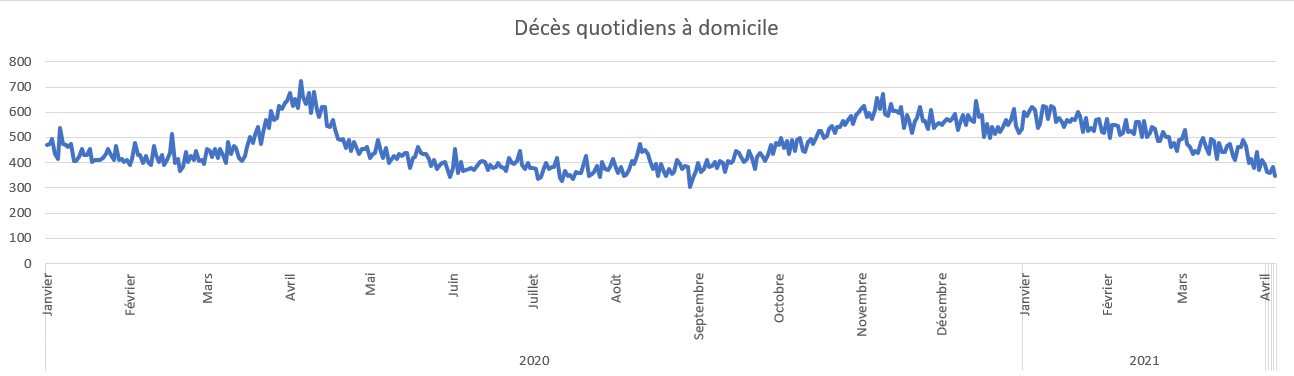
\includegraphics[width=10.41667in,height=\textheight]{data/images/domicile.png}

Ce résultat de non-prise en charge peut expliquer le caractère
particulier des données de Chypre.

\includegraphics[width=10.41667in,height=\textheight]{gen/images/deceshebdochyprelissage.png}

De la même manière qu'en France, où l'on constate un nombre de décès
inscrits à l'état civil plus important les lundis et mardis et très
faibles les dimanches, à Chypre la fin du confinement n'est probablement
pas liée à un excès mortalité, mais plutôt à la découverte tardive des
décès non répertoriés.

\hypertarget{la-mortalituxe9-des-infections-respiratoires-aiguuxebs-telle-que-la-covid-19}{%
\paragraph{2.3.2 La mortalité des infections respiratoires aiguës telle
que la
Covid-19}\label{la-mortalituxe9-des-infections-respiratoires-aiguuxebs-telle-que-la-covid-19}}

La période de mars-avril est extrêmement particulière dans toute
l'histoire du soin, car il s'agit de la première fois que l'on demande à
des malades de ne pas consulter de généraliste, en particulier si le
patient souffre d'une infection respiratoire.

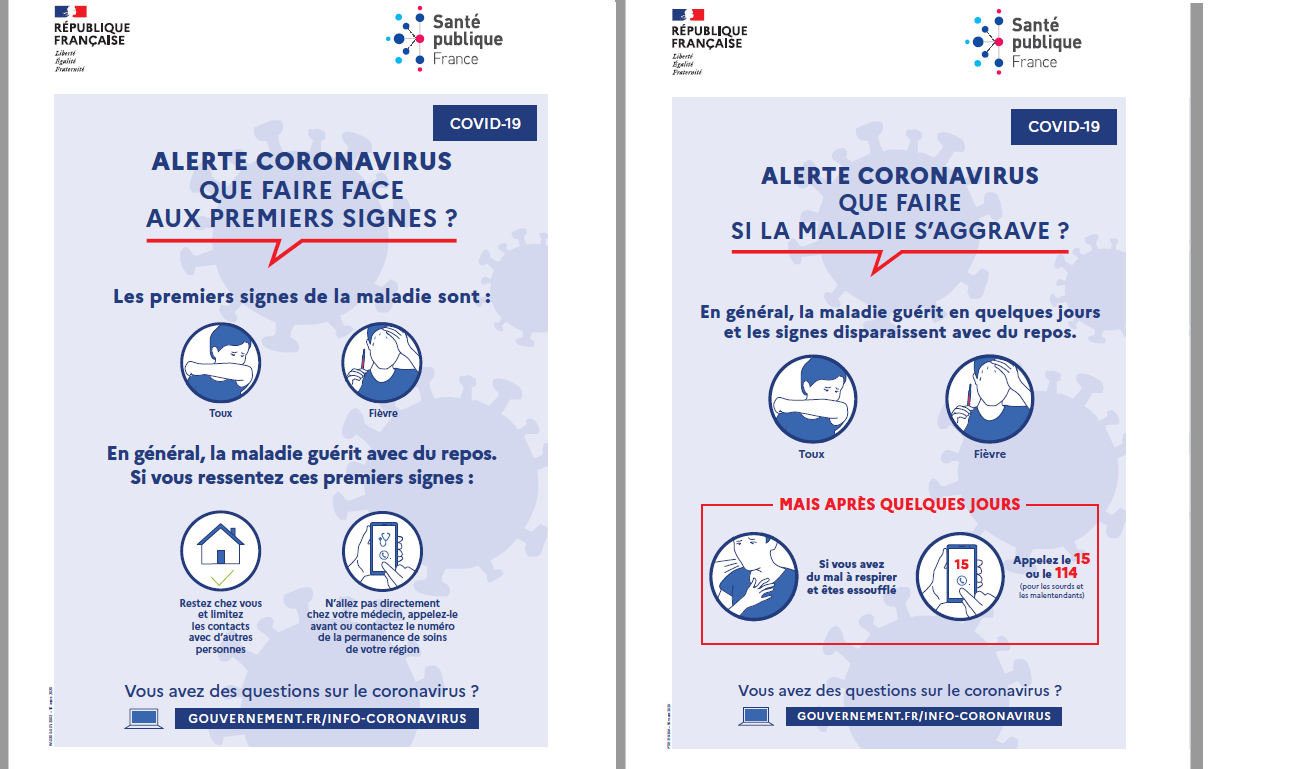
\includegraphics[width=10.41667in,height=\textheight]{data/images/flyerspf.png}

Cet ordre a entraîné un comportement de la population inédit dont on
peut voir les effets sur les statistiques d'achat de médicaments en
pharmacie de la base de données Médicam.

Ce graphique représente la base remboursable de tous les médicaments
vendus par les pharmacies en France, chaque mois.

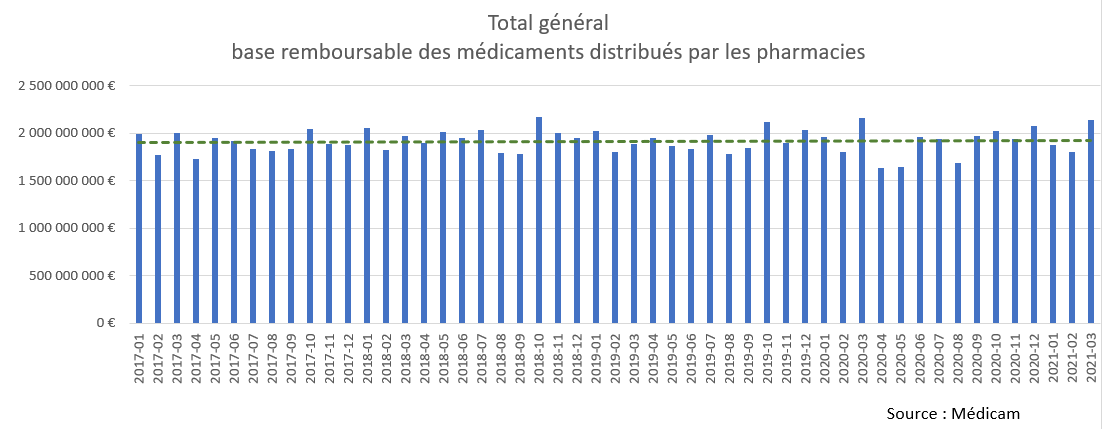
\includegraphics[width=10.41667in,height=\textheight]{data/images/medictot.png}

Le mois de mars 2020 a connu une hausse de 13~\% des ventes de
médicaments par rapport à la moyenne 2017-2019, représentant le
provisionnement des français à la suite de l'annonce du confinement
généralisé. Les mois d'avril et mai 2020 présentent au contraire, des
baisses de 15~\% et 14~\% par rapport à la moyenne. Ces baisses sont le
reflet de la non-prescription par les médecins à la suite de l'ordre de
ne pas consulter.

Cette chute est cependant bien plus forte concernant les traitements
habituels prescrits dans le cadre des infections respiratoires aiguës.
En particulier les antibiotiques permettant d'éviter les surinfections
ont connu une chute sans précédent.

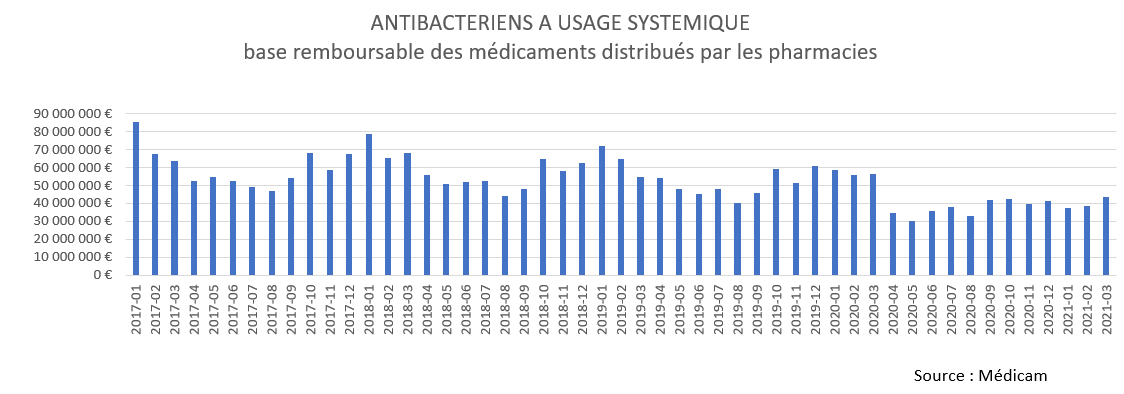
\includegraphics[width=10.41667in,height=\textheight]{data/images/medicbac.png}

En mars, le provisionnement n'a pas existé et le total d'antibiotiques
vendus est inférieur de 1~\% à la moyenne 2017-2019. En avril et mai,
les chutes de ventes furent respectivement de 40~\% et 47~\%. Depuis
cette période, la vente d'antibiotiques est restée à des niveaux
extrêmement bas, reflet du choix de ne pas proposer ce traitement en cas
de Covid-19.

Ce choix de ne pas laisser les médecins de ville proposer de traitements
dans le cadre d'une infection respiratoire aiguë pendant les mois de
mars et d'avril, a entraîné une dégradation sans précédent de l'état de
santé des patients. La non-prescription d'antibiotiques aura permis aux
bactéries de proliférer chez les patients âgés et affaiblis. Ainsi, à
partir de fin mars, de nombreux français dont l'état de santé s'est
dégradé à leur domicile affluent dans les services hospitaliers. Les
coronavirus, comme la Covid-19, ont pu entraîner des lésions dans
l'appareil respiratoire empêchant les patients de respirer. Ces lésions
sont également des portes ouvertes aux surinfections bactériennes. Les
sujets âgés se présentant à la l'hôpital ont à la fois des « trous »
dans les poumons les empêchant de respirer, mais également des bactéries
se développant à la suite de ces lésions et de la chute des défenses
immunitaires. Ces 2 pathologies combinées empêchent de répondre
rapidement aux besoins du patient. Si une injection de corticoïdes
pouvait permettre au patient de réparer les trous des poumons, elle
accélèrerait la prolifération des bactéries, entraînant la mort par
surinfection. A l'inverse, ne pas agir sur la mécanique respiratoire
entraîne le décès du patient dans les plus brefs délais. De nombreux
patients sont décédés non pas à cause du caractère exceptionnel de la
maladie, mais à cause du caractère exceptionnel de la situation~: pas de
prise en charge précoce, et pas de traitement antibiotique.

Une fois de plus, pour les personnes les plus pauvres et vivant dans les
logements les moins salubres, pour lesquelles nous avons vu plus haut
une plus forte hausse de mortalité, il est normal qu'un confinement à
domicile forcé engendre une probabilité plus importante de souffrir
d'une infection, que le manque d'antibiotique ne manquera pas de laisser
s'aggraver.

Ce défaut de prise en charge a été quantifié par les deux membres du
Conseil Scientifique, Arnaud Fontanet et Simon Cauchemez, pourtant à
l'origine de cette stratégie. Leur article dans Science \footnote{\url{https://science.sciencemag.org/content/369/6500/208}},
utilise les données hospitalières françaises et notamment le temps de
passage et réanimation et de décès depuis la prise en charge du patient.
Les courbes les plus intéressantes ont été supprimés depuis de l'article
principal, mais sont toujours disponibles dans les données
complémentaires. Au pages 15 et 16 sont détaillés les nombres de jours
que mettent les patients arrivant à l'hôpital avant d'aller en
réanimation (graphique de gauche) et le nombre de jours qu'ils mettent
avant de décéder (graphique de droite).

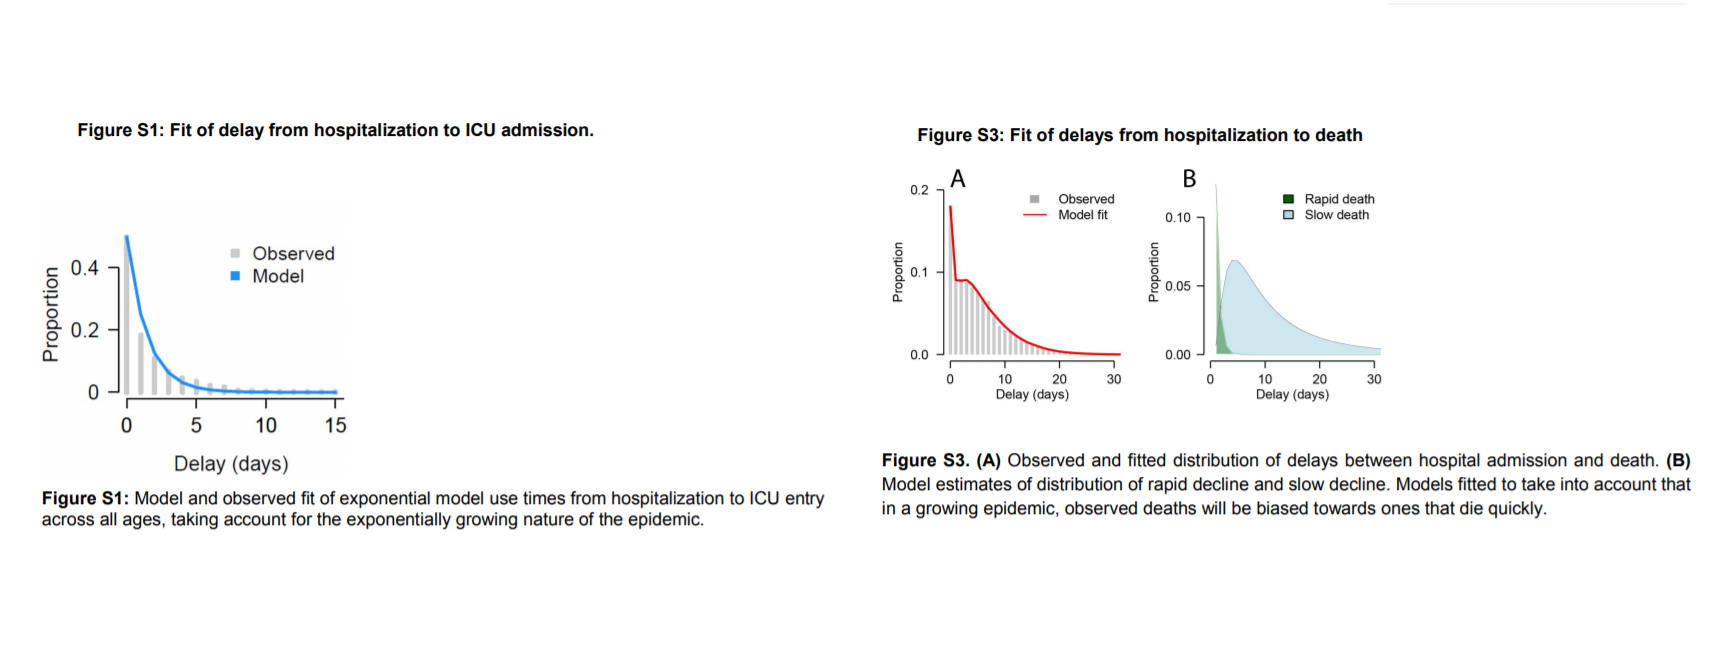
\includegraphics[width=10.41667in,height=\textheight]{data/images/fontanet.png}

Ainsi, 50~\% des patients arrivant à l'hôpital sont placés en
réanimation dès de le premier jour et 17\% des patients décèdent dès le
premier jour. Ces ratios énormes prouvent que les patient arrivent trop
tard à l'hôpital. On observe d'ailleurs une très forte différence entre
le nombre de décès au jour 1 et le nombre de décès au jour 2, illustrant
qu'une grosse partie des arrivées n'est plus sauvable. Les auteurs en
déduisent d'ailleurs qu'il y a 2 courbes séparés entre ceux arrivant
trop tard et les autres. C'est l'explication restante dans l'article
toujours en ligne. Une lecture moins orientée déduit de cet énorme ratio
de décès au premier jour que les soins sont trop tardifs. Il est donc
très probable que les décédés des jours suivants soient également pour
beaucoup du fait de personnes dont l'état a eu le temps de s'aggraver et
dont certain auraient pu survivre si les soins avaient été précoces. Ces
17\% de patients arrivés trop tard représentent 3~000~personnes sur les
17~570~décès déclarés Covid-19 à l'hôpital sur cette période. Si on
considère qu'un décès dans les 3~jours à l'hôpital est un signe d'une
prise en charge trop tardive, le total de décès potentiellement évitable
est alors de 6~000.

Dans la vidéo ``100~000 morts, vraiment ?''\footnote{\url{https://www.youtube.com/watch?v=MLMGnfeu_zk}},
nous détaillons par lieu les décès durant cette période pour trouver que
la surmortalité à l'hôpital pendant l'épisode de mars-avril est de
6~000~personnes. Ainsi la surmortalité constatée est égale au nombre de
décès précoces de l'hôpital entraînés par la non prise en charge des
patients de façon précoce par les médecins de ville.

\hypertarget{laccuxe9luxe9ration-artificielle-des-duxe9cuxe8s}{%
\paragraph{2.3.3 L'accélération artificielle des
décès}\label{laccuxe9luxe9ration-artificielle-des-duxe9cuxe8s}}

L'article 12-3 du chapitre 7 du Décret n° 2020-293 du 23 mars 2020
prescrivant les mesures générales nécessaires pour faire face à
l'épidémie de Covid-19 dans le cadre de l'état d'urgence sanitaire
décrète une dérogation au code de la santé publique \footnote{\url{https://www.legifrance.gouv.fr/loda/id/LEGIARTI000041767762/2020-03-29/}}
:

\begin{verbatim}
    la spécialité pharmaceutique Rivotril ® sous forme injectable peut faire l'objet d'une dispensation, jusqu'au 15 avril 2020, par les pharmacies d'officine en vue de la prise en charge des patients atteints ou susceptibles d'être atteints par le virus SARS-CoV-2 dont l'état clinique le justifie sur présentation d'une ordonnance médicale portant la mention “ Prescription Hors AMM dans le cadre du covid-19 ”.
\end{verbatim}

Le Rivotril est un médicament antiépileptique dont l'utilisation n'a
haibtuellement rien à voir les infections respiratoires, ni
l'accompagnement palliatif par sédation. Dans la notice du vidal
\footnote{\url{https://www.vidal.fr/medicaments/gammes/rivotril-8874.html}},
il est mentionné comme contre-indications :

\begin{verbatim}
Ce médicament ne doit pas être utilisé dans les cas suivants :

    insuffisance respiratoire grave,

    syndrome d'apnée du sommeil,

    insuffisance hépatique grave,

    myasthénie.
\end{verbatim}

Ainsi, la dérogation du décret ne propose pas l'utilisation d'un
sédatif, mais d'un médicament déclenchant l'arrêt de la respiration du
patient et donc son décès anticipé. Le décret a eu cours du 28 mars au
11 mai, soit dans la période exacte sur laquelle est constatée le plus
fort nombre de décès depuis la canicule de 2003. L'analyse des ventes de
Rivotril en pharmacie dans sa forme injectable reflète l'ampleur de
l'utilisation de ce produit.

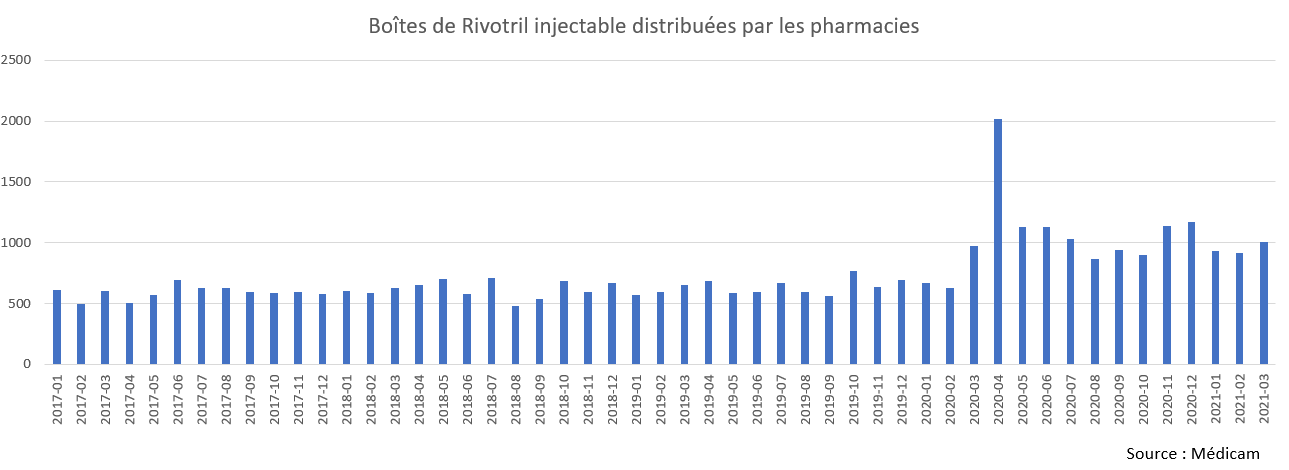
\includegraphics[width=10.41667in,height=\textheight]{data/images/rivotril.png}

Ainsi, contrairement aux antibiotiques, les ventes de boîtes Rivotril
dans a forme injectable ont augmenté de 59~\% au mois de mars et de
227~\% en avril relativement à la moyenne observée entre 2017 et 2019.
Cette augmentation sur mars-avril représente 1 700 boîtes du produit et
plus de l'habitude. Précisons que chaque boîte contient 6 ampoules dont
une à 2 sont utilisées par patient dans le cadre d'une fin de vie. Ces
statistiques ne reflètent que partiellement l'utilisation de cette
molécule, car elles ne prennent pas en compte les doses qui ne sont pas
distribuées par les pharmacies de ville, par exemple en provenance
directe de l'hôpital. On s'étonne par la suite que la consommation de ce
produit dans sa forme injectable n'ait pas retrouvé son ancien niveau.
Entre mars 2020 et mars 2021, ce sont 6 150 boîtes supplémentaires à
l'habitude qui ont été vendues, soit plus de 36 000 ampoules.

La comparaison des décès déclarés Covid \footnote{\url{https://www.data.gouv.fr/fr/datasets/donnees-relatives-a-lepidemie-de-covid-19-en-france-vue-densemble/}}
et des décès toutes causes dans les EHPADs présente ainsi des
incohérences massives. Celles-ci sont détaillées dans la vidéo précitée.
Par exemple autour du 31 mars, la quasi-totalité des décès des EHPADs
sont enregistrées dans les statistiques Covid alors que moins de la
moitié des régions françaises connaissent une surmortalité et sont
considérées touchées par cette pathologie.

L'origine de ce comptage de peut aisément s'expliquer à la lumière de ce
choix palliatif.

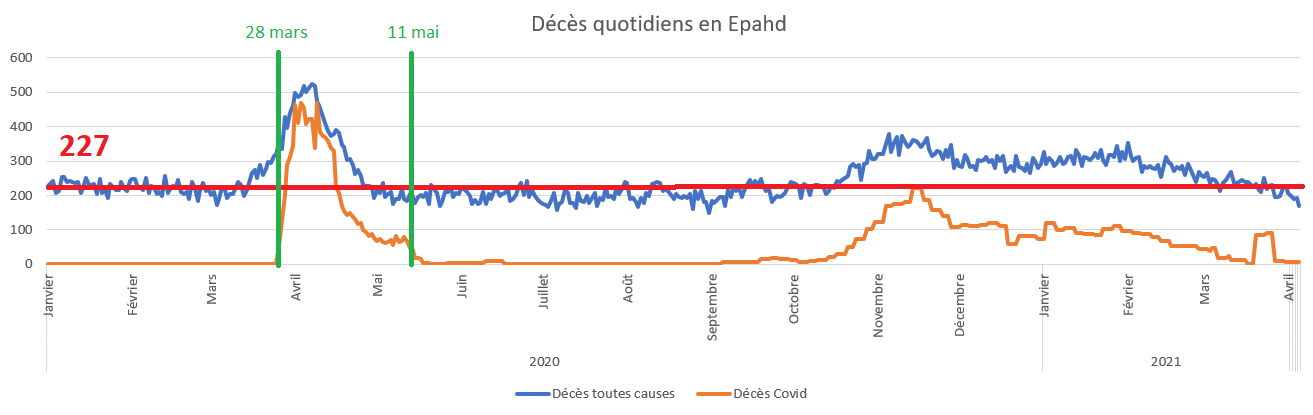
\includegraphics[width=10.41667in,height=\textheight]{data/images/EHPAD.png}
On constate que les remontées de décès Covid arrivent massivement après
la promulgation du décret dérogatoire concernant le Rivotril. De plus,
même après la fin de la période de surmortalité française à partir du
1er mai, des décès Covid ont bien été enregistrés dans les EHPADs
jusqu'à la fin de la validité du décret.

Il est évident qu'une intervention médicamenteuse ayant pour conséquence
d'accélérer le décès de patients en fin de vie, a des répercussions sur
les statistiques de décès. Dès lors, la ``surmortalité'' constatée sur
courte période n'est pas le signe d'un plus grand nombre de décès à
moyen terme, mais uniquement d'un regroupement artificiel de décès sur
les mêmes dates.

Cette intervention médicamenteuse mériterait d'être quantifiée à
l'hôpital. Si un nombre significatif de patient a ``bénéficié'' de la
mesure dérogatoire le premier jour d'arrivée à l'hôpital, il devient
tout à fait normal d'avoir ce pic significatif de décès ce premier jour.

\hypertarget{le-pic-de-mortalituxe9-pruxe9coce-doctobre-2020}{%
\subsubsection{2.4 Le pic de mortalité précoce d'octobre
2020}\label{le-pic-de-mortalituxe9-pruxe9coce-doctobre-2020}}

De nombreux pays européens présentent une mortalité saisonnière forte et
précoce dès octobre 2020. Seuls quelques pays échappent à cette hausse
des décès : Chypre, Malte, le Danemark, l'Islande, la Norvège et la
Finlande. Pour les pays concernés cependant, la hausse de mortalité est
simultanée, rendant, encore une fois, impossible la seule cause d'un
unique virus se propageant en Europe. Nous notons de surcroît, que la
généralisation du port du masque, les gestes barrière, les fermetures de
nombreux lieux publics, les jauges de publics dans les commerces, la
profusion de gel hydroalcoolique ou encore la diffusion du télétravail,
n'ont absolument pas empêché la mortalité hivernale d'être aux mêmes
niveaux, voire légèrement supérieur à ce qui est observé d'habitude. Il
s'agit d'un indice supplémentaire qu'elle n'est aucunement liée à un
phénomène de propagation.

Il s'agit alors de comprendre pourquoi, fin 2020, les habitants d'une
majorité de pays européens semblent en moins bonne santé que les autres
années. Les périodes de stress, le manque de sortie peuvent être des
éléments favorisant la faiblesse des défenses immunitaires. En France,
comme dans une grande parte des pays européens, une très vaste campagne
de vaccination grippale a eu lieu à partir d'octobre 2020. Le taux de
couverture vaccinale a gagné presque 10 points en 2020 par rapport aux
années précédentes \footnote{\url{https://www.santepubliquefrance.fr/determinants-de-sante/vaccination/articles/donnees-regionales-de-couverture-vaccinale-grippe-par-saison-et-dans-chaque-groupe-d-age}}.

La campagne de vaccinale grippale arrive tardivement dans l'année. Elle
est concomitante à la hausse de mortalité hivernale.

\includegraphics[width=10.41667in,height=\textheight]{gen/images/vaccins_distribues.png}

Les débats sont ouverts sur l'utilité réelle du vaccin contre la grippe
sur la mortalité hivernale. Rappelons que ce vaccin n'est pas conçu
comme les autres. Il s'agit d'un mélange contenant plusieurs souches de
grippes préconisés par l'OMS. Au moment de la préconisation, absolument
aucune certitude n'existe sur les souches qui circuleront pendant
l'hiver. Il s'agit donc d'un pari. Certains pays comme la Norvège ou la
Finlande en ont une distribution plus faible que d'autres, en
particulier depuis les polémiques ayant suivi la campagne vaccinale
contre le virus H1N1. Pour autant, la Norvège et la Finlande semblent ne
pas être soumis à des pics de mortalités hivernales ces dernières
années, bien au contraire. Les données disponibles sur les vaccins ne
sont disponibles que mensuellement, ne permettant pas un rapprochement
de qualité avec les décès en France. Un lissage hebdomadaire des vaccins
distribués comparé aux décès toutes causes des plus de 65 ans en France
(population la plus vaccinée du fait de la gratuité à cet âge), montre
une proximité entre ces 2 évènements.

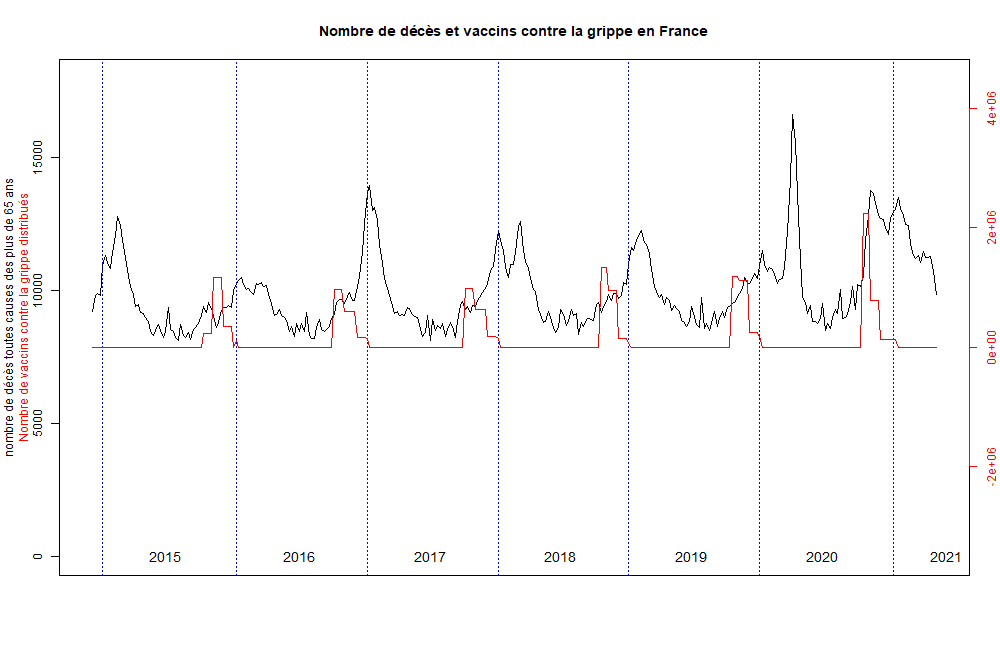
\includegraphics[width=10.41667in,height=\textheight]{data/images/lien_deces_grippe.png}

La hausse soudaine des décès en octobre 2020 comparativement aux années
précédentes correspond en dates et proportions aux observations du
passé. Même si corrélation n'est pas causalité, les soupçons à ce niveau
devraient soulever des recherches poussées complémentaires. Il serait
nécessaire de comparer les dates de décès de tous les français depuis
2015, aux dates de vaccinations. Il s'agirait de déterminer si un lien
statistique existe entre date de vaccination et date de décès. Les
données précises et nominatives des décès de tous les français sont
publiques et disponibles en ligne. Le rapprochement avec les dates de
vaccinations devrait être possible pour les chercheurs disposant des
droits d'accès aux données de vaccinations.

Les liens entre vaccinations et détérioration temporaire des défenses
immunitaires ont pourtant déjà fait l'objet d'études. Une étude de
janvier 2020 \footnote{\url{https://www.ncbi.nlm.nih.gov/pmc/articles/PMC7126676/}}
montre des liens statistiques entre la vaccination grippale et une
augmentation du nombre de malades des autre pathologies, en particulier
les coronavirus. Si on ajoute le fait que pendant l'hiver 2019-2020, la
mortalité attribuée à la grippe est proche de 0, il paraît
contradictoire de lancer en octobre 2020 une campagne de vaccination
d'une ampleur jamais égalée contre une maladie qui ne paraît pas si
mortelle. Les impacts du seul effet nocébo \footnote{\url{https://pharmacomedicale.org/66-pharmacologie/medicaments-alternatifs/placebo/161-toxicite-effet-nocebo}}devrait
engendrer un débat contradictoire sur l'oppoortunité d'une opération à
grande échelle concernant la grippe dans un contexte de ``guerre''
affichée contre ``un'' coronavirus. Chaque personne ayant été vacciné a
déjà été prévenu des effets indésirables des vaccins sur l'organisme.
Les notices des vaccins disponibles sur le Vidal\footnote{\url{https://www.vidal.fr/medicaments/gammes/vaxigriptetra-79276.html}}
préviennent de l'ensemble de ces effets ainsi que de leur (haute)
fréquence.

Pour conclure, il est nécessaire de rappeler à ce stade qu'en France,
cette hausse de mortalité intervient dans un contexte de 2e confinement
dont nous avons détaillé les effets plus haut, ainsi que dans une
consommation historiquement basse d'antibiotiques.

Il convient alors de se demander aussi si l'augmentation de la mortalité
visible à partir d'octobre provient comme relayé politiquement par la
presse, d'un seul virus qui se déclencherait partout en même temps, ou
de l'effet combiné de la dégradation cyclique de l'état de santé combiné
à des mesures favorisant la survenue précoce de maladies hivernales
telles que les coronavirus, avec une dégradation de la qualité des
soins.

\hypertarget{le-rebond-de-mortalituxe9-depuis-duxe9but-2021}{%
\subsubsection{2.5 Le rebond de mortalité depuis début
2021}\label{le-rebond-de-mortalituxe9-depuis-duxe9but-2021}}

Il n'est pas exceptionnel d'avoir autour du 1er janvier de chaque année,
deux périodes de hausse de mortalité visibles. C'est notamment le cas en
France pendant l'hiver 2017-2018. Cependant ces périodes sont
habituellement très rapprochées dans le temps. En 2021, pour certains
pays, le deuxième pic de mortalité est fortement éloigné du premier.
Pour la première fois, en 2021, une politique sanitaire d'une ampleur
jamais égalée, à partir de vaccins expérimentaux sur lesquels aucun
recul n'est disponible, a été décidé. Ce dispositif fait lui aussi
l'objet d'un suivi hors norme. De nombreux pays envoient leurs données
de vaccinations en quasi direct \footnote{\url{https://ourworldindata.org/covid-vaccinations}}.
Il est difficile d'avoir une idée précise de la qualité des remontées de
données, mais il offre des possibilités de comparaisons jamais égalées.

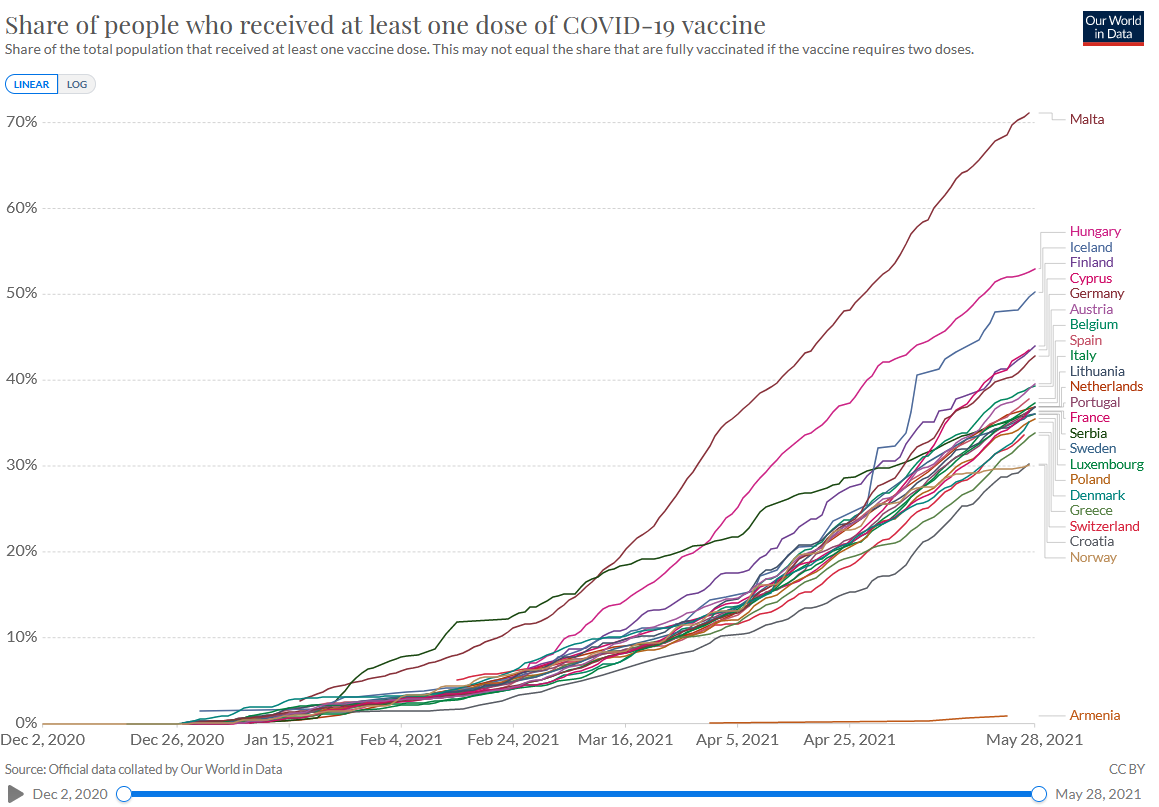
\includegraphics[width=10.41667in,height=\textheight]{data/images/ourworldindata.png}

En particulier, Malte et la Hongrie déclarent une vaccination à très
grande échelle sur leur territoire. Ainsi, les vaccinations concernent
des jeunes depuis plusieurs semaines.

\hypertarget{la-hongrie-pays-test-de-la-politique-vaccinale-uxe0-grande-uxe9chelle}{%
\paragraph{2.5.1 La Hongrie, pays test de la politique vaccinale à
grande
échelle}\label{la-hongrie-pays-test-de-la-politique-vaccinale-uxe0-grande-uxe9chelle}}

Concernant la Hongrie, on note une concomitance parfaite entre le début
de la campagne vaccinale contre la Covid-19 et une très forte hausse de
la mortalité pour atteindre le maximum connu en décembre pour les plus
de 65 ans. Pour les moins de 65 ans, la situation est pire que 2 mois
auparavant. Il s'agit même d'un record absolu pour toute la période où
nous disposons de données sur Eurostat (2013).

\includegraphics[width=10.41667in,height=\textheight]{gen/images/decesvaccinhongrie.png}

Le focus sur le moins de 40 ans qui ne décèdent que très peu lors des
épisodes hivernaux confirme ce résultat.

\includegraphics[width=10.41667in,height=\textheight]{gen/images/decesvaccinhongriejeune.png}

Si on prend en compte l'évolution de la pyramide des âges en Hongrie et
la forte baisse du nombre de moins de 40 ans, il s'agit également de la
période connaissant le plus de décès de jeunes enregistrés. Etant
communément admis que les jeunes ne décèdent quasiment jamais
d'infections respiratoires aiguës contractées pendant l'hiver, et pas
plus de la Covid-19, le nombre de causes possibles de cette surmortalité
est limitée. Même si certains affirmeront que la cause viendrait d'un
nouveau virus, cela signifierait qu'il serait apparu uniquement depuis
la campagne vaccinale.

Les semaines 10 à 17 en Hongrie ont enregistré 485 décès de personnes de
moins de 40 ans. A la même époque, en 2020, 355 décès seulement ont été
enregistrés, soit une hausse historique de 36\%. Ces décès sont
parfaitement indétectables par les méthodes de suivis habituels
concernant les médicaments. La Hongrie possède 4,35 millions d'habitants
de moins de 40 ans. Une surmortalité de 130 personnes représente dans la
population 0,0002964\%. Si l'on avait suivi un échantillon de 10 000
hongrois de moins de 40 ans, nous n'aurions trouvé aucun mort
supplémentaire. Seuls les poisons violents peuvent être détectés par ce
type de pratique.

La pharmacovigilance ne permet pas non-plus de suivre efficacement les
liens entre l'administration d'un produit et la mortalité qui suivrait.

En premier lieu, le suivi des données est inadapté. D'une part, la
pharmacovigilance est passive. Les institutions attendant que des
individus (patients, professionnels de santé\ldots) notifient les cas à
la pharmacovigilance de l'ANSM ou du fabricant. Cependant, il est
notoire que cette attente passive ne fonctionne pas et que les remontées
sont bien plus rares que les cas, ce qu'on appelle la sous notification.
Les études sur le sujet estiment que seulement 1~\% des évènements
indésirables sont rapportés, donc que 99\% ne sont jamais connus
\footnote{\url{https://digital.ahrq.gov/ahrq-funded-projects/electronic-support-public-health-vaccine-adverse-event-reporting-system},\url{https://www.ncbi.nlm.nih.gov/pmc/articles/PMC4368609/}}.
Dans le cas présent, on peut estimer qu'environ seulement 1 décès d'une
personne de moins de 40 ans a pu remonter à la pharmacovigilance
hongroise.

Enfin, la méthode d'imputabilité utilisée ne permet pas de lier le décès
à l'administration d'un vaccin. Cette méthode s'appuie sur le principe
Challenge - Déchallenge - Rechallenge\footnote{\url{https://pharmacomedicale.org/images/desc2016/Methodes_dimputabilite_-_DES_Pharmaco_Med_-_24112016.pdf}}.
Ainsi, un effet devient identifié entre un produit et un évènement
indésirable, lorsque que l'évènement est arrivé arpès la prise du
produit (par exemple une éruption cutanée), puis que l'évènement s'est
arrêté après l'arrêt de la prise du produit (fin de l'éruption cutanée)
et enfin que l'évènement est revenu après la reprise du produit
(nouvelle éruption cutanée). Dans le cas présent, un décès d'un jeune de
moins de 40 suite à l'administration de la première dose ne pourra
rentrer que dans la cas ``Challenge''. Il n'est pas possible de
réveiller un mort pour lui administrer une seconde dose et vérifier
qu'il décède de nouveau. Un tel cas serait dons codifié comme peu
probant.

Dès lors, la seule façon de détecter la létalité d'une intervention est
malheureusement de le faire après la difffusion de cette dernière à
grande échelle, par une étude de mortalité toute cause, comme la
présente étude.

\hypertarget{luxe9tude-des-autres-pays-europuxe9ens-confirment-lanalyse}{%
\paragraph{2.5.2 L'étude des autres pays européens confirment
l'analyse}\label{luxe9tude-des-autres-pays-europuxe9ens-confirment-lanalyse}}

La situation est similaire à Malte. le niveau de décès est important en
2021, mais surtout, il concerne cette fois des moins de 65 ans. Le
faible nombre d'habitant de Malte ne permet toutefois pas de descendre
au niveau des moins de 40 ans (il décède à Malte en moyenne 2 personnes
de moins de 40 ans par semaine).

\includegraphics[width=10.41667in,height=\textheight]{gen/images/decesvaccinmalte.png}

En Islande, pays qui n'a pourtant pas connu d'épisode de surmortalité en
2020, une vaccination extrêmement massive a été effectuée en quelques
jours. Ce pic de vaccination est parfaitement synchronisé a un pic de
mortalité.

\includegraphics[width=10.41667in,height=\textheight]{gen/images/decesvaccinislande.png}

A l'inverse du côté des pays n'ayant que peu mis en place une politique
vaccinale, le nombre de décès reste calme. Pour la Norvège, pays ayant
le moins vacciné ses habitants, la mortalité n'a connue qu'un léger
rebond depuis le début de la campagne de vaccination.

\includegraphics[width=10.41667in,height=\textheight]{gen/images/decesvaccinnorvege.png}

Pour les jeunes également, la mortalité reste à son niveau bas, même si
on note une dynamique en augmentation.

\includegraphics[width=10.41667in,height=\textheight]{gen/images/decesvaccinnorvegejeune.png}
La Croatie, a peu vacciné comme la Norvège, mais a regroupé la majorité
de sa campagne vaccinale sur les mêmes jours. On constate un pic de
mortalité concomitant à la vaccination.

\includegraphics[width=10.41667in,height=\textheight]{gen/images/decesvaccincroatie.png}

A l'instar de la Norvège, la situation chez les jeunes semble dans la
norme. Rappelons ici que les campagnes vaccinales visent en premier chef
les personnes âgées.

\includegraphics[width=10.41667in,height=\textheight]{gen/images/decesvaccincroatiejeune.png}

Pour la quasi-totalité des pays d'Europe dont nous disposons des
données, il apparaît nettement une reprise de la mortalité
(cf.~annexes). Il convient alors de se poser la question du ratio
bénéfices/risques de la politique actuelle.

\hypertarget{une-politique-sanitaire-dont-on-questionne-les-liens-avec-la-santuxe9}{%
\subsection{Une politique sanitaire dont on questionne les liens avec la
santé}\label{une-politique-sanitaire-dont-on-questionne-les-liens-avec-la-santuxe9}}

Nous observons que la mortalité observée depuis un peu plus d'un an
partout en Europe est à un niveau comparable au reste de notre décennie.
Il existe des variations entre les différents Etats, mais le lien entre
les politiques affichées et le niveau de mortalité ne semble pas
évident, voire dans le sens inverse de l'attendu. Pour la France, les
différentes mesures identifiées participent mécaniquement à une
augmentation des décès sans que l'on puisse quantifier un quelconque
impact bénéfique. Dès lors, si la mortalité n'est finalement pas
exceptionnelle, est-il raisonnable d'entretenir un climat de peur, de
maintenir les règles liberticides en place et de lancer des campagnes de
vaccinations d'une ampleur jamais connue réalisées à partir de produits
expérimentaux ? Nous observons que les campagnes de vaccination en
période hivernale sont liées à des augmentations de mortalité. Il
conviendrait d'analyser en profondeur ce lien avant de continuer à
promouvoir des produits dans des périodes où la santé des européens
baisse cycliquement. Nous observons que tous les pays européens ayant
démarré en masse une campagne de vaccination contre la Covid-19 ont des
taux de mortalité inhabituels pour la saison. Les pays ayant le plus
massivement vaccinés ont des taux de mortalité chez leurs jeunes jamais
égalés jusqu'à maintenant.

Est-il raisonnable de continuer cette politique sanitaire inconnue dans
ces conditions ? N'est-il pas urgent de reprendre le cours normal des
consultations pour retrouver l'usage des médicaments que nous avions
avant 2020 avec une mortalité plus faible au lieu de faire le pari de
l'efficacité de nouveaux produits miracles ?

Enfin, cette analyse est une analyse statistique. Aucune analyse
statistique ne permet jamais d'obtenir une certitude. C'est d'ailleurs
l'arme utilisé en permanence par tous les producteurs pour se défendre
contre les plaignants ayant perdu un proche. Il appartient à chaque fois
au juge de se contenter d'une vraisemblance de causalité en revenant à
du ``bon sens'' pour statuer\footnote{\url{https://www.lexbase.fr/revues-juridiques/61548960-jurisprudence-monsanto-et-les-sept-peches-capitaux-epilogue-de-la-saga-du-lasso-par-la-condamnation}}.
Jamais nous ne pourrons être ``certains'' par l'analyse des
statistiques, ni de la dangerosité de la Covid-19, ni du vaccins. Jamais
même, nous ne pourrons être certains de la qualité et de l'exactitude
des données que nous manipulons.

Cependant, si nous ne sommes pas sûrs du lien de causalité entre la
vaccination massive en cours et la hausse de la mortalité, alors nous ne
sommes pas sûrs non plus du lien de causalité entre la remontée de tests
positifs Covid-19 et la hausse mortalité.

Si nous ne sommes pas sûrs de la qualité des données de mortalité, alors
la nouvelle politique sanitaire ne repose sur aucune base solide.
Inversement, si nous sommes sûrs de la qualité des données de mortalité,
alors leur analyse approfondie montre qu'il faut cesser immédiatement la
stratégie actuelle.

Dans tous les cas, il est urgent de retrouver ce qui manque cruellement
depuis plus d'un an, et qui doit primer devant tout le reste : du bon
sens.

\hypertarget{annexes}{%
\section{Annexes}\label{annexes}}

\hypertarget{les-duxe9cuxe8s-hebdomadaires-par-pays}{%
\subsection{Les décès hebdomadaires par
pays}\label{les-duxe9cuxe8s-hebdomadaires-par-pays}}

\hypertarget{pays-pruxe9sentant-un-pic-de-mortalituxe9-en-mars-avril}{%
\subsubsection{Pays présentant un pic de mortalité en
mars-avril}\label{pays-pruxe9sentant-un-pic-de-mortalituxe9-en-mars-avril}}

\includegraphics[width=10.41667in,height=\textheight]{gen/images/deceshebdofrancelissage.png}
\includegraphics[width=10.41667in,height=\textheight]{gen/images/deceshebdobelgiquelissage.png}

\includegraphics[width=10.41667in,height=\textheight]{gen/images/deceshebdosuisselissage.png}
\includegraphics[width=10.41667in,height=\textheight]{gen/images/deceshebdoespagnelissage.png}

\includegraphics[width=10.41667in,height=\textheight]{gen/images/deceshebdoitalielissage.png}
\includegraphics[width=10.41667in,height=\textheight]{gen/images/deceshebdoluxembourglissage.png}

\includegraphics[width=10.41667in,height=\textheight]{gen/images/deceshebdopaysbaslissage.png}

\includegraphics[width=10.41667in,height=\textheight]{gen/images/deceshebdosuedelissage.png}
\includegraphics[width=10.41667in,height=\textheight]{gen/images/deceshebdochyprelissage.png}

\hypertarget{pays-ne-pruxe9sentant-pas-de-pic-de-mortalituxe9-en-mars-avril-2020}{%
\subsubsection{Pays ne présentant pas de pic de mortalité en mars-avril
2020}\label{pays-ne-pruxe9sentant-pas-de-pic-de-mortalituxe9-en-mars-avril-2020}}

\includegraphics[width=10.41667in,height=\textheight]{gen/images/deceshebdoportugallissage.png}

\includegraphics[width=10.41667in,height=\textheight]{gen/images/deceshebdomaltelissage.png}

\includegraphics[width=10.41667in,height=\textheight]{gen/images/deceshebdoautrichelissage.png}
\includegraphics[width=10.41667in,height=\textheight]{gen/images/deceshebdohongrielissage.png}
\includegraphics[width=10.41667in,height=\textheight]{gen/images/deceshebdobulgarielissage.png}
\includegraphics[width=10.41667in,height=\textheight]{gen/images/deceshebdortchequelissage.png}
\includegraphics[width=10.41667in,height=\textheight]{gen/images/deceshebdodanmarklissage.png}
\includegraphics[width=10.41667in,height=\textheight]{gen/images/deceshebdoestonielissage.png}
\includegraphics[width=10.41667in,height=\textheight]{gen/images/deceshebdocroatielissage.png}
\includegraphics[width=10.41667in,height=\textheight]{gen/images/deceshebdoislandelissage.png}
\includegraphics[width=10.41667in,height=\textheight]{gen/images/deceshebdolichtensteinlissage.png}
\includegraphics[width=10.41667in,height=\textheight]{gen/images/deceshebdolettonielissage.png}
\includegraphics[width=10.41667in,height=\textheight]{gen/images/deceshebdomontenegrolissage.png}
\includegraphics[width=10.41667in,height=\textheight]{gen/images/deceshebdonorvegelissage.png}
\includegraphics[width=10.41667in,height=\textheight]{gen/images/deceshebdopolognelissage.png}
\includegraphics[width=10.41667in,height=\textheight]{gen/images/deceshebdoserbielissage.png}
\includegraphics[width=10.41667in,height=\textheight]{gen/images/deceshebdoslovaquielissage.png}
\includegraphics[width=10.41667in,height=\textheight]{gen/images/deceshebdoslovenielissage.png}
\includegraphics[width=10.41667in,height=\textheight]{gen/images/deceshebdoallemagnelissage.png}
\includegraphics[width=10.41667in,height=\textheight]{gen/images/deceshebdoalbanielissage.png}

\includegraphics[width=10.41667in,height=\textheight]{gen/images/deceshebdogrecelissage.png}
\includegraphics[width=10.41667in,height=\textheight]{gen/images/deceshebdofinlandelissage.png}
\includegraphics[width=10.41667in,height=\textheight]{gen/images/deceshebdoroumanielissage.png}

\includegraphics[width=10.41667in,height=\textheight]{gen/images/deceshebdoarmenielissage.png}

\hypertarget{les-duxe9cuxe8s-confrontuxe9s-uxe0-la-vaccination-covid-par-pays}{%
\subsection{Les décès confrontés à la vaccination Covid par
pays}\label{les-duxe9cuxe8s-confrontuxe9s-uxe0-la-vaccination-covid-par-pays}}

\includegraphics[width=10.41667in,height=\textheight]{gen/images/decesvaccinhongrie.png}
\includegraphics[width=10.41667in,height=\textheight]{gen/images/decesvaccinmalte.png}
\includegraphics[width=10.41667in,height=\textheight]{gen/images/decesvaccinfrance.png}
\includegraphics[width=10.41667in,height=\textheight]{gen/images/decesvaccinislande.png}
\includegraphics[width=10.41667in,height=\textheight]{gen/images/decesvaccinchypre.png}
\includegraphics[width=10.41667in,height=\textheight]{gen/images/decesvaccinallemagne.png}
\includegraphics[width=10.41667in,height=\textheight]{gen/images/decesvaccinautriche.png}

\includegraphics[width=10.41667in,height=\textheight]{gen/images/decesvaccinbelgique.png}

\includegraphics[width=10.41667in,height=\textheight]{gen/images/decesvaccinsuisse.png}

\includegraphics[width=10.41667in,height=\textheight]{gen/images/decesvaccinespagne.png}

\includegraphics[width=10.41667in,height=\textheight]{gen/images/decesvaccinpaysbas.png}

\includegraphics[width=10.41667in,height=\textheight]{gen/images/decesvaccinpologne.png}
\includegraphics[width=10.41667in,height=\textheight]{gen/images/decesvaccindanmark.png}
\includegraphics[width=10.41667in,height=\textheight]{gen/images/decesvaccinsuede.png}

\includegraphics[width=10.41667in,height=\textheight]{gen/images/decesvaccingrece.png}

\includegraphics[width=10.41667in,height=\textheight]{gen/images/decesvaccincroatie.png}
\includegraphics[width=10.41667in,height=\textheight]{gen/images/decesvaccinnorvege.png}
\includegraphics[width=10.41667in,height=\textheight]{gen/images/decesvaccinserbie.png}

\hypertarget{les-duxe9cuxe8s-quotidiens-par-duxe9partement-franuxe7ais}{%
\subsection{Les décès quotidiens par département
français}\label{les-duxe9cuxe8s-quotidiens-par-duxe9partement-franuxe7ais}}

\includegraphics[width=10.41667in,height=\textheight]{gen/images/BourgogneFrancheComté.png}
\includegraphics[width=10.41667in,height=\textheight]{gen/images/AuvergneRhôneAlpes.png}
\includegraphics[width=10.41667in,height=\textheight]{gen/images/PaysdelaLoire.png}
\includegraphics[width=10.41667in,height=\textheight]{gen/images/PACA.png}
\includegraphics[width=10.41667in,height=\textheight]{gen/images/ÎledeFrance.png}
\includegraphics[width=10.41667in,height=\textheight]{gen/images/NouvelleAquitaine.png}
\includegraphics[width=10.41667in,height=\textheight]{gen/images/HautsdeFrance.png}
\includegraphics[width=10.41667in,height=\textheight]{gen/images/GrandEst.png}
\includegraphics[width=10.41667in,height=\textheight]{gen/images/Occitanie.png}
\includegraphics[width=10.41667in,height=\textheight]{gen/images/ÎledeFrance.png}
\includegraphics[width=10.41667in,height=\textheight]{gen/images/Corse.png}
\includegraphics[width=10.41667in,height=\textheight]{gen/images/Bretagne.png}
\includegraphics[width=10.41667in,height=\textheight]{gen/images/CentreValdeLoire.png}

\end{document}
